\chapter{Praktische Evaluation} \label{sec:evaluation}

\section{Testumgebung}
Die folgenden Experimente wurden auf mithilfe einer AMD EPYC 7763 64-Core CPU mit 16 nutzbaren Hardwarethreads und 64GB Arbeitsspeicher durchgeführt. Das System
verwendet Ubuntu 24.04 als Betriebssystem und GCC in der Version 13.2.0 als Compiler. Die Algorithmen wurden in C++20 implementiert und mit der Optimierungsstufe
\texttt{-O3} kompiliert. Die Ausführung der Algorithmen mit einer spezifischen Anzahl von Threads wurde softwareseitig über OpenMP-Instruktionen (\cite{openmp}) realisiert. 

\section{Implementierung}

\subsection{Klassenstruktur}
\begin{figure}[ht]
    \centering
    \caption{Klassenstruktur der Implementierung}
    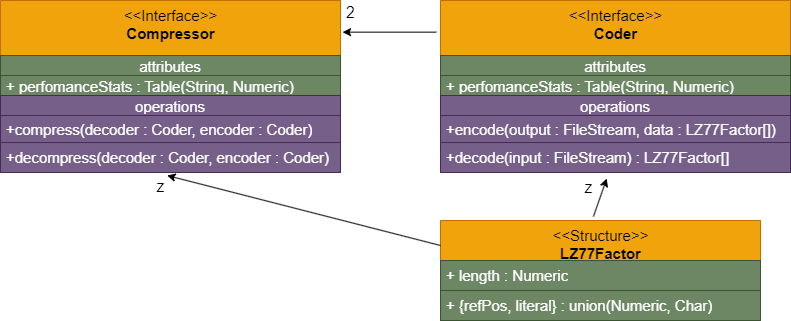
\includegraphics[scale=0.4]{Images/uml.png} \label{uml}
\end{figure}

Die in \ref{uml} dargestellte Klassenstruktur illustriert die grundlegende Abstraktion, die für die Implementierung der Algorithmen verwendet wurde. Compressor und
Coder beschreiben jeweils ein Interface bzw. ein Template, welches durch ein konkretes Kompressionsverfahren und einer Kodierung spezialisiert werden kann. Jegliche
Spezialisierungen teilen sich jedoch eine gemeinsame Definition eines Faktors im LZ77-Schema.

\subsection{Externe Bibliotheken}
Im Folgenden werden die genutzten externen Bibliotheken aufgelistet, die im Rahmen der Implementierung der Algorithmen, sowie deren Evaluation genutzt wurden.
\subsubsection{Malloc Count} \label{malloccount}
Malloc Count (\cite{malloc_count}) ist eine C++-Bibliothek, die es ermöglicht, Speicherallokationen und -freigaben auf dem Heap zu überwachen und zu messen. Im
Rahmen unserer Evaluation gibt uns diese Bibliothek die Spitze des allokierten Speichers innerhalb der Ausführung der Algorithmen aus.

\subsubsection{Unordered-Dense-Map} \label{unordereddense}
Die Unordered-Dense-Map (\cite{unordered_dense}) stellt eine performante Hashtabelle dar, die insbesondere in der Dauer ihrer Suchoperationen gegenüber
der std::unordered\_map aus der Standardbibliothek deutlich trumpft. Dies Hashtabelle wurde in Approx.LZ77 und Approx.LZ77Par für die Speicherung der
RFPs in jeder Runde verwendet. Im Rahmen der Entwicklung von Approx.LZ77Par hat sich die Verwendung mehrerer Instanzen von Unordered-Dense-Map im Vergleich
zu anderen inherent parallelen Hashtabellen (\cite{oneapi}) (\cite{sharded_map}) als effizienter herausgestellt.

\subsubsection{LibSaiS}
Für die Implementierung der exakten LZ77-Faktorisierung, die als Referenzalgorithmus fungiert, wurde die Bibliothek LibSaiS (\cite{libsais}) zu Hilfe genommen. Diese
Bibliothek stellt eine effiziente Implementierung für die Konstruktion des Suffix-Arrays bereit.

\subsubsection{STL - Sortierung}
Die Standardbibliothek von C++ stellt bereits Implementierungen von Sortieralgorithmen bereit. Diese wurden in der Implementierung von LZ77 und Approx.LZ77 für
die nachträgliche Sortierung der Faktoren verwendet. Insbesondere wurden Execution Policies (\cite{execpol}) genutzt, um die Sortierung parallelisieren zu können.

\subsection{Parametrisierte Einstellung}
Die folgenden Einstellungen definieren eine Kalibrierung von Approx. LZ77 und Approx. LZ77Par in der jeweils optimierten(opt) bzw. unoptimierten(unopt) Variante. 
Die Einstellungen für beide Varianten sind in der Tabelle \ref{settings} aufgeführt.

\begin{table} [ht]
    \centering
    \caption{Parameter und Einstellung für die unoptimierte(unopt) und optimierte(opt) Ausführung von Approx.LZ77}
    \label{settings}
    \begin{tabular}{|c|c|c|}
        \hline
        \textbf{Einstellung} & \textbf{unopt} & \textbf{opt} \\
        \hline
        DynEnd & Deaktiviert & $r_{DynEnd}=26$ \\
        \hline
        DynStart & Deaktiviert & Aktiv \\
        \hline
        PreMatching & Deaktiviert & $r_{PreMatch}=23$ \\
        \hline
        ScanSkip & $k_{min}=0\%$ & $k_{min}=3\%$ \\
        \hline
    \end{tabular}
\end{table}

Falls nicht anders ausgewiesen, wurden die Approximationsalgorithmen in der opt-Variante mit den in Tabelle \ref{settings} festgelegten Parametern ausgeführt. In der
Ausführung von Approx.LZ77Par wurde die Ausführung standardmäßig mit 16 Threads durchgeführt.

\section{Messung}

\subsection{Eingabedaten}
Die folgenden Algorithmen wurden auf verschiedenen Dateien aus dem Pizza \& Chili-Corpus (\cite{corpus}) getestet. Die verwendeten Dateien decken verschiedene Kontexte und damit
Kompressionspotentiale ab.
\begin{table}[ht]
    \centering
    \caption{Auflistung der verwendeten Eingabedaten aus dem Pizza \& Chili-Corpus(\cite{corpus}}
    \label{inputdata}
    \begin{tabular}{|c|c|c|c|c|}
        \hline
        \textbf{Datei} & \textbf{Größe} & \textbf{Alphabetgröße} & \textbf{Beschreibung} \\
        \hline
        \texttt{dna} & 200MB & 4 & DNA-Sequenzen \\
        \hline
        \texttt{english} & 200MB & 256 & Englische Texte \\
        \hline
        \texttt{proteins} & 200MB & 20 & Proteinsequenzen \\
        \hline
        \texttt{sources} & 200MB & 256 & Quellcode \\
        \hline
        \texttt{xml} & 200MB & 256 & XML-Dateien \\
        \hline
    \end{tabular}
\end{table}
In der Tabelle \ref{inputdata} sind die verwendeten Dateien aufgelistet. Die Größe der Dateien wurde auf 200MB beschränkt, um einen angemessenen Rahmen für die 
Laufzeitmessung zu erhalten. Detaillierte Messungen werten wir auf der Eingabe proteins aus, da diese Datei die schlechtesten Metriken aufweist. Weitergehende
Laufzeitmessungen der anderen Dateien sind in \ref{alternative} aufgeführt.

\subsection{Messgrößen}

\subsubsection{Laufzeit}
Die Laufzeit der Algorithmen wurde innerhalb der Ausführung gemessen. Dabei wird die Zeitmessung nach dem Laden der Eingabedatei gestartet und mit dem vollständigen
Auffüllen einer Faktorfolge beendet. Damit wird das Einlesen der Eingabe und eine eventuelle Kodierung der Ausgabe nicht in die Laufzeitmessung einbezogen. Diese Strategie
hat ihren Hintergrund in der Tatsache, dass die konkrete Ausprägung des Eingabe- und Ausgabestroms keine Aussagekraft über die Qualität der Kompression hat.

\subsubsection{Speicher}
Der Speicherverbrauch der Algorithmen wurde auch intern mithilfe einer externen Bibliothek \ref{malloccount} gemessen. Dabei wurden Speicherallokationen auf dem Heap 
überwacht und gemessen. Im Rahmen dieser Arbeit wurde die Spitze des allokierten Speichers im Zeitraum nach dem Einlesen der Eingabedatei und nach dem vollständigen 
Auffüllen der Faktorfolge gemessen. Zu Vergleichszwecken wird der Speicherverbrauch in Relation zur Eingabegröße angegeben.

\subsubsection{Kompressionsrate CR*} \label{cr}
Die Kompressionsrate wird neben der Anzahl der Faktoren zum Großteil von der verwendeten Kodierung bestimmt. Wie bereits erwähnt, sind wir in der Wahl der Kodierung
nicht beschränkt, sodass die Aussagekraft bezüglich der Qualität der Kompression eingeschränkt ist. Es ist jedoch zu beachten, dass Faktoren, die durch Approx.LZ77
erzeugt werden stets eine Zweierpotenz als Länge annehmen. Die binäre Repräsentation dieser Längen kann daher in Abhängigkeit von der gewählten Kodierung kompakt 
konstruiert werden. Um dieses Phänomen zu illustrieren, geben wir im Folgenden eine naive Kodierung vor, auf dessen Grundlage wir die Kompressionrate $CR^*$ definieren.
\begin{equation}
    |K^{LZ77}_{OUT}(f)| = 1 + \begin{cases}
        2\log_2(n) & \text{falls } |f| > 1 \\
        8 & \text{sonst}
    \end{cases}
\end{equation}
Im Falle von LZ77 bestimmt ein Bit, ob es sich um eine Referenz oder ein einzelnes Zeichen handelt. Im Falle einer Referenz wird die Länge und die Position der Referenz
mithilfe von $\log_2(n)$ Bits kodiert. Im Falle eines einzelnen Zeichens wird die ASCII-Kodierung des Zeichens verwendet, die 8 Bits benötigt.
\begin{equation}
    |K^{Approx.LZ77}_{OUT}(f)|= 1 + \begin{cases}
        \log_2(n)+\log_2(\log_2(n)) & \text{falls } |f| > 1 \\
        8 & \text{sonst}
    \end{cases}
\end{equation}
Im Falle von Approx.LZ77 kann die Länge mithilfe von $\log_2(\log_2(n))$ Bits kodiert werden, da die Länge anhand einer einzelnen Bitposition bestimmt wird.
In Anlehnung an die Größe der verwendeten Testdaten erhalten wir für die Optimierung, DynEnd, die folgende Endrunde:
\begin{equation}
    r_{DynEnd} = \lceil log_2{|S|}-log_2{\lceil\frac{Min^{Ref}_{Bin}}{Max^{Lit}_{Bin}}\rceil} \rceil = 26
\end{equation}

\newpage
\subsection{Messwerte}

\begin{table}[ht]
    \centering
    \caption{Messwerte der Algorithmen auf verschiedenen Eingabedateien}
    \label{messwerte}
    \begin{tabular} { |c|c|c|c|c|c|c| }
        \hline
        \textbf{Eingabe} & \textbf{Algorithmus} & \textbf{Laufzeit[s]} & \textbf{Speicher} & $\mathbf{FR_{unopt}}$ & \textbf{FR} & \textbf{CR*} \\
        \hline
        & LZ77 & 15.76 & 14.88 & & 9.95\% & 70.92\% \\
        proteins & Approx.LZ77 & 44.06 & 9.94 & 15.07\% & 15.34\% & 63.95\% \\
        & Approx.LZ77Par & 6.99 & 10.21 & 15.07\% & 15.34\% & 63.95\% \\
        \hline
        & LZ77 & 13.79 & 13.44 & & 5.50\% & 39.20\% \\
        sources & Approx.LZ77 & 40.43 & 6.42 & 9.64\% & 10.05\% & 40.14\% \\
        & Approx.LZ77Par & 6.49 & 5.90 & 9.64\% & 10.05\% & 40.14\% \\
        \hline
        & LZ77 & 15.32 & 13.44 & & 6.66\% & 47.45\% \\
        english & Approx.LZ77 & 51.00 & 7.06 & 10.22\% & 10.42\% & 43.39\% \\
        & Approx.LZ77Par & 7.46 & 6.16 & 10.22\% & 10.42\% & 43.39\% \\
        \hline
        & LZ77 & 14.91 & 13.44 & & 6.66\% & 47.46\% \\
        dna & Approx.LZ77 & 30.10 & 8.38 & 10.67\% & 10.71\% & 45.53\% \\
        & Approx.LZ77Par & 4.80 & 6.66 & 10.67\% & 10.71\% & 45.53\% \\
        \hline
        & LZ77 & 13.21 & 12.72 & & 3.35\% & 23.89\% \\
        xml & Approx.LZ77 & 29.38 & 3.46 & 6.41\% & 6.62\% & 26.78\% \\
        & Approx.LZ77Par & 4.91 & 3.46 & 6.41\% & 6.62\% & 26.78\% \\
        \hline
    \end{tabular}
\end{table}

\begin{figure}[H]
    \centering
    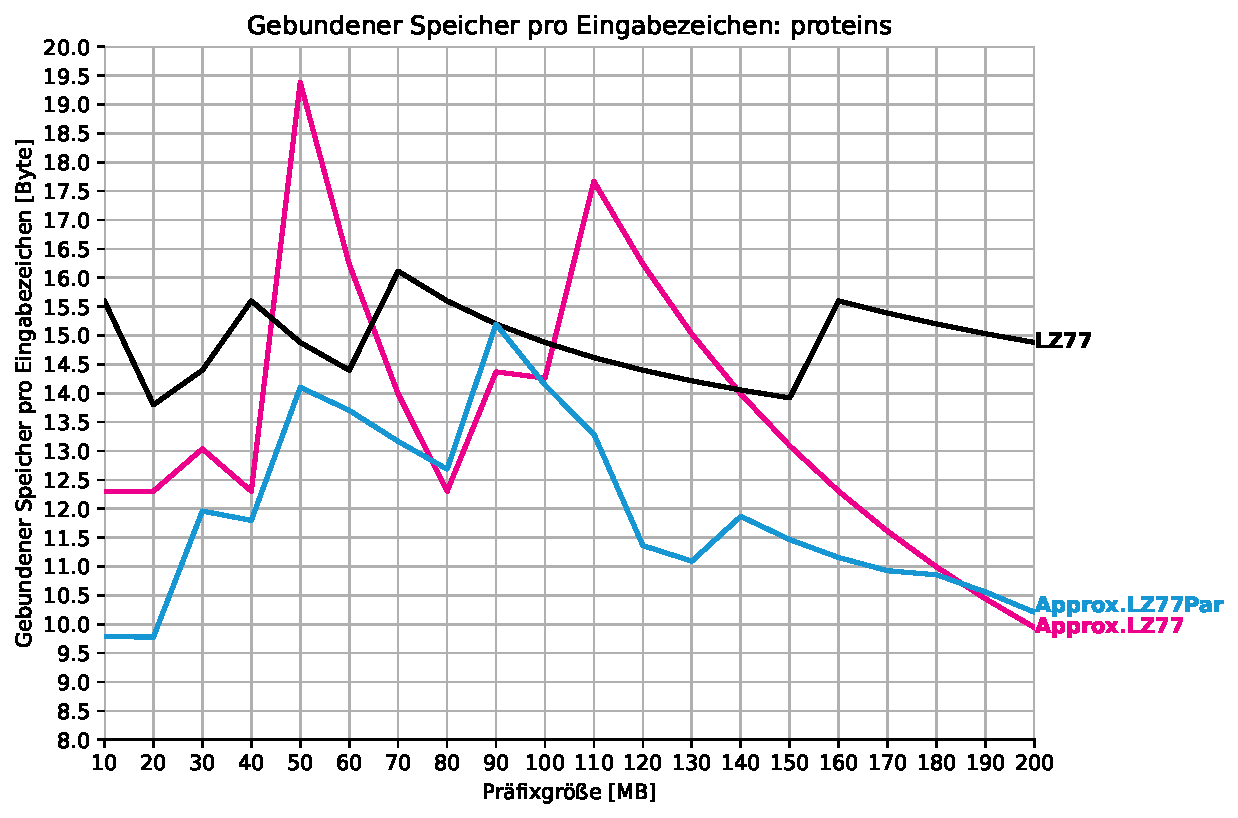
\includegraphics[scale=0.65]{Images/progressive_mem.pdf}
    \caption{Speicherverbrauch von LZ77, Approx.LZ77 und Approx.LZ77Par(16 Threads) auf verschiedenen Präfixen von proteins. Aufgezeichnet wurde das Verhältnis
    von allokiertem Speicher zur Eingabegröße.}
    \label{memory}
\end{figure}

\begin{figure}[H]
    \centering
    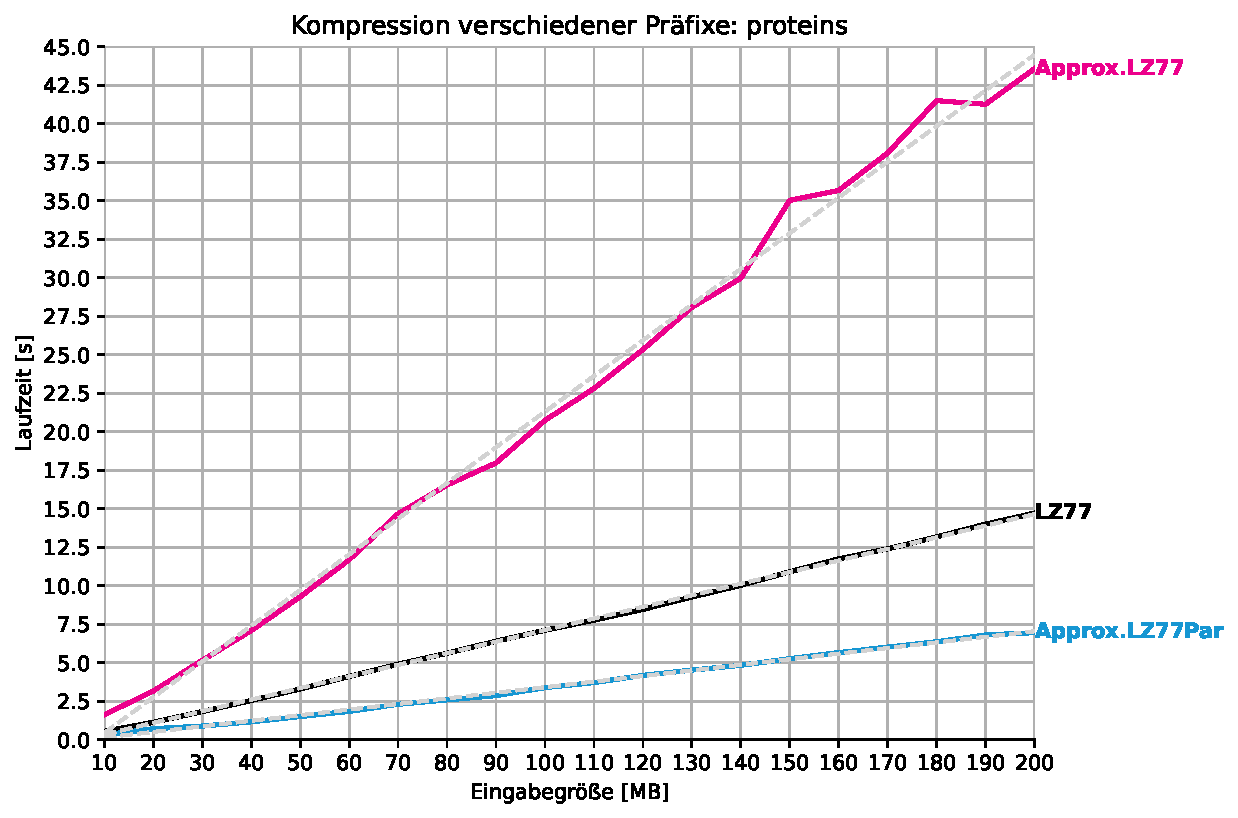
\includegraphics[scale=0.65]{Images/progressive_proteins.pdf}
    \caption{Laufzeitmessung von LZ77, Approx.LZ77 und Approx.LZ77Par(16 Threads) auf verschiedenen Präfixen von proteins. Als Vergleichsmaß wurde 
    die lineare Regression der Kurven gestrichelt eingezeichnet.}
    \label{runtime}
\end{figure}
    
\begin{figure}[H]
    \centering
    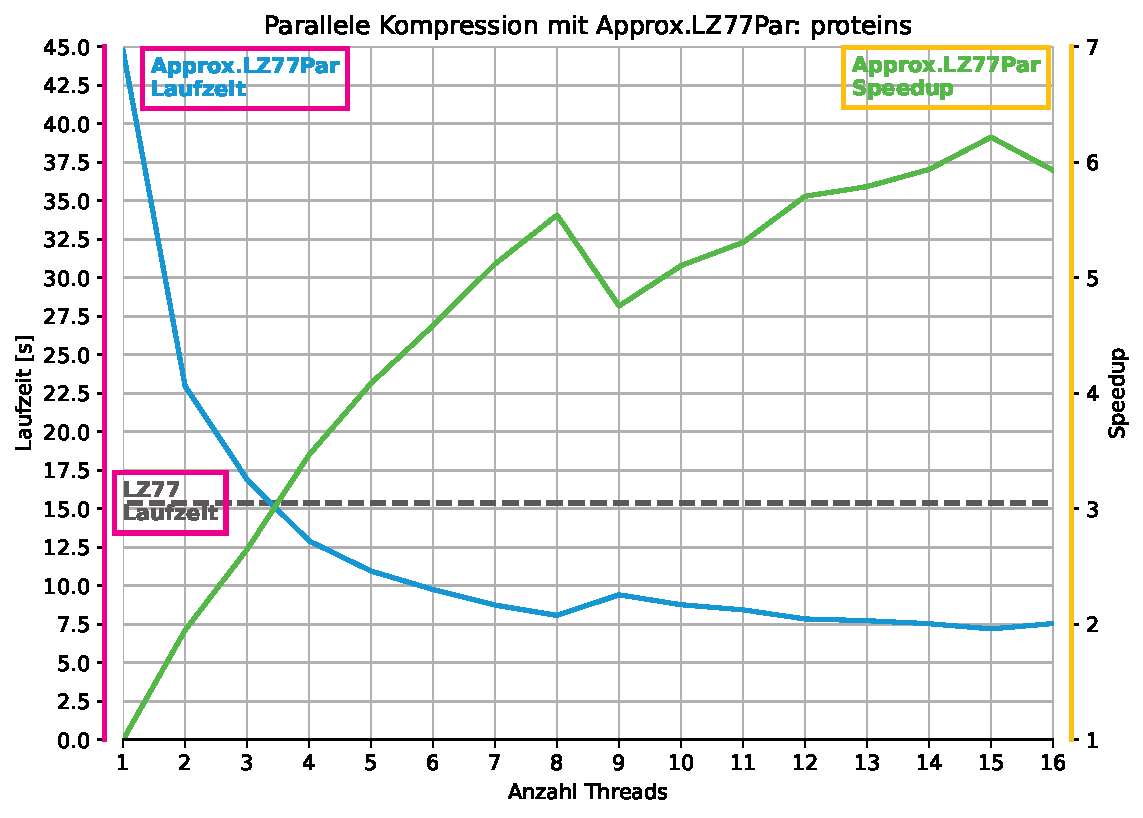
\includegraphics[scale=0.65]{Images/progressive_speedup_proteins.pdf}
    \caption{Laufzeit-(Blau) und Speedup(Grün)-Messung von Approx.LZ77Par mit verschiedener Anzahl an Threads für proteins}
    \label{runtime_threads}
\end{figure}

\begin{figure}[H]
    \centering
    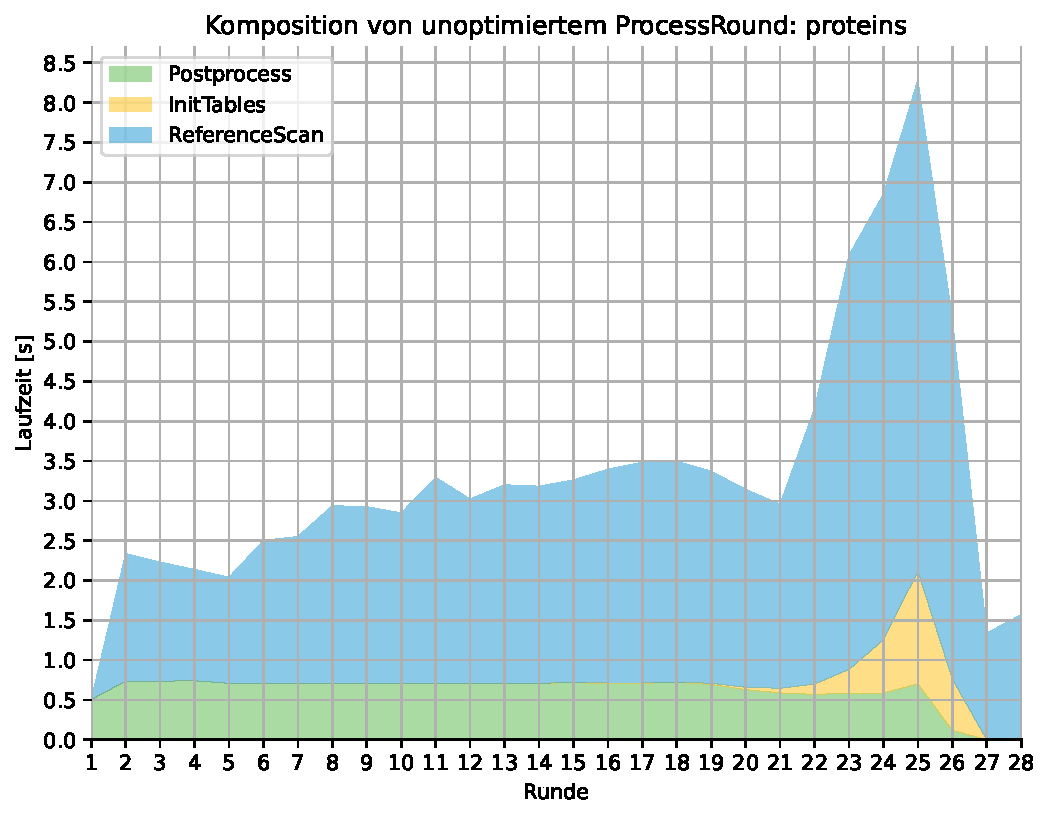
\includegraphics[scale=0.63]{Images/progressive_unopt_stack.pdf}
    \caption{Darstellung der Verteilung der Laufzeit der Subroutinen innerhalb jeder Runde im Falle einer Ausführung von Approx.LZ77 ohne jegliche Optimierungen \ref{settings}.
    Postprocess deckt dabei die nötigen Prozesse zum Rundenübergang, wie das Spalten der Blöcke und der Extraktion der Faktoren, ab.}
    \label{unopt}
\end{figure}

\begin{figure}[H]
    \centering
    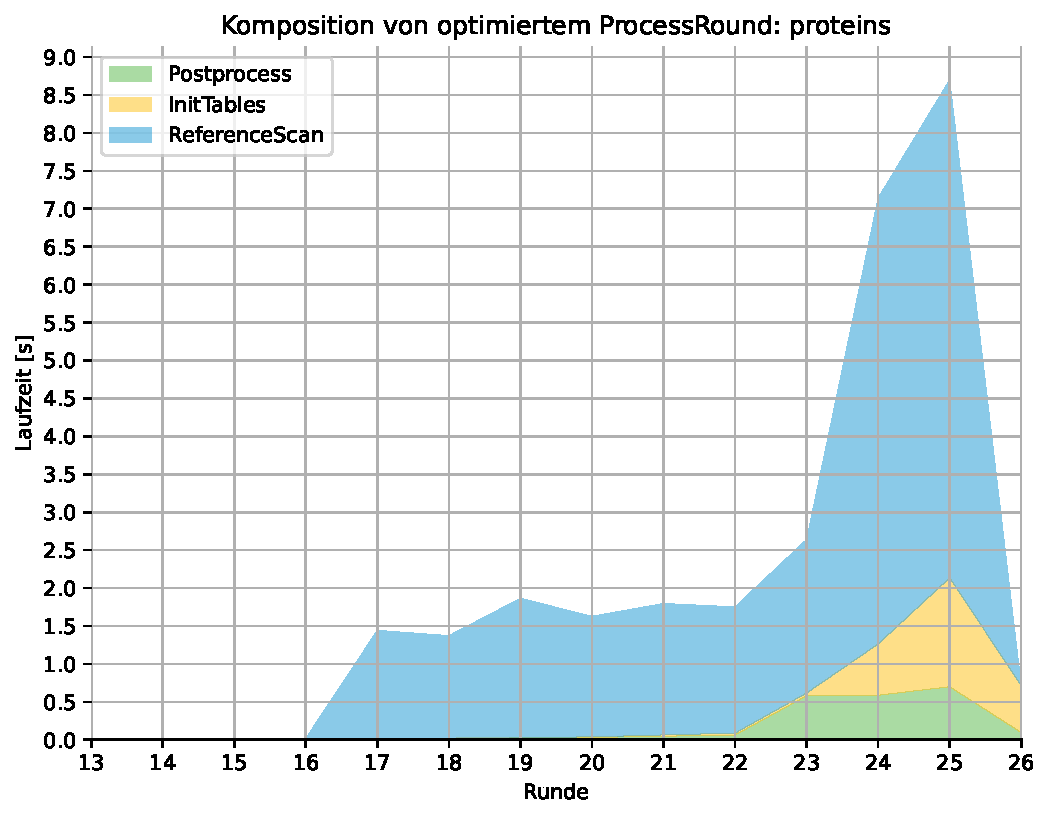
\includegraphics[scale=0.63]{Images/progressive_opt_stack.pdf}
    \caption{Darstellung der Verteilung der Laufzeit der Subroutinen innerhalb jeder Runde im Falle einer Ausführung von Approx.LZ77 mit allen Optimierungen \ref{settings}.
    Postprocess deckt dabei die nötigen Prozesse zum Rundenübergang, wie das Spalten der Blöcke und der Extraktion der Faktoren, ab.}
    \label{opt}
\end{figure}

\section{Auswertung}
\subsection{LZ77}
Wie in Kapitel 3.1 beschrieben, zeigt der verwendete Algorithmus zur Generierung einer exakten LZ77-Faktorisierung ein lineares Verhalten bezüglich der Laufzeit.
Dies wird in Abbildung \ref{runtime} deutlich, wo die Laufzeitmessung von LZ77 auf verschiedenen Präfixen von proteins dargestellt ist. Die lineare Regression der
Laufzeit deckt sich mit der tatsächlichen Laufzeitmessung. Auch in Bezug auf die Speichernutzung wird die theoretische Analyse bestätigt. In Abbildung \ref{memory}
ist der Speicherverbrauch von LZ77 auf verschiedenen Präfixen von proteins aufgezeichnet. Der in Kapitel 3.1 beschriebene Speicherverbrauch von 12 Byte pro Eingabezeichen
stellt auch für die Messwerte eine untere Schranke dar. Der zusätzliche Speicherverbrauch ist durch die Speicherung der Faktoren bestimmt, die in die Messung einfließen.
Hiermit konnten wir die theoretische Analyse des Laufzeit- und Speicherverhaltens empirisch bestätigen.

\subsection{Approx. LZ77}
In \ref{messwerte} wird deutlich, dass Approx. LZ77 dem exakten LZ77-Algorithmus in der Laufzeit und der Faktorrate stets deutlich unterlegen ist. Wie bereits in Kapitel
3.2 beschrieben, liegt der Fokus von Approx. LZ77 auf der Reduktion des Speicherverbrauchs. In der theoretischen Abschätzung der Laufzeiten wurde bereits festgestellt,
dass Approx. LZ77 eine schlechtere Laufzeitkomplexität als LZ77 aufweist. Im Rahmen des Speicherbedarfs zeigt sich, dass Approx. LZ77 in den meisten Fällen eine geringere
Speichernutzung aufweist als LZ77. In Relation zur Eingabegröße verfügt Approx. LZ77 jedoch eine hohe Varianz in der Speichernutzung. Dies stellt eine Konsequenz der
theoretischen Abschätzung der Speichernutzung dar, die insbesondere eine hohe Abhängigkeit von der Größe der Faktorfolge aufweist. In Abbildung \ref{memory} wird 
ebenfalls deutlich, dass selbst verschiedene Präfixe einer Eingabedatei unterschiedliche relative Speichernutzungen aufweisen. Dies lässt sich auf ein 
unterschiedliches Maß der Redundanz in den Eingaben zurückführen. Die Kompressionsrate $CR^*$ von Approx. LZ77 ist in \ref{messwerte} ebenfalls aufgeführt. Es ist 
zu erkennen, dass die Abweichung der Kompressionsrate von LZ77 in den meisten Fällen geringer ausfällt als die Abweichung der Faktorrate. Dies ist auf die in 
\ref{cr} beschriebene Eigenart der Kodierung zurückzuführen.

\subsection{Approx. LZ77 Optimierungen}
Die praktischen Optimierungen aus Kapitel 3.4 wurden in der Evaluation von Approx. LZ77 und Approx. LZ77Par standardmäßig aktiviert. Um den Nutzen dieser Optimierungen
zu verdeutlichen wurden in \ref{unopt} und \ref{opt} die Auswirkungen auf die Laufzeiten der einzelnen Runden von Approx.LZ77 aufgezeichnet. Aufgrund der 
Optimierungen DynStart und DynEnd ist sofort ersichtlich, dass der Algorithmus einen großen Anteil der sonst nötigen Runden auslässt. Konkret werden die ersten 12 und
die letzten 2 Runden im Falle der Eingabe proteins ausgelassen. Dies bringt bereits eine signifikante Reduktion der Gesamtlaufzeit. Die Postprocess-Routine umfasst hier 
die Prozesse, die im Rundenübergang stattfinden, wie das Spalten der Blöcke und die explizite Extraktion der Faktoren.
Weiterhin fällt auf, dass die InitTables- und Postprocess-Routine im optimierten Fall deutlich weniger Zeit in Anspruch nehmen.  Dies lässt sich auf die Anwendung von 
PreMatching zurückführen, da Blöcke in InitTables vorgefiltert werden und so weniger Einfügeoperationen stattfinden, sowie im Rundenübergang die Spaltung der Blöcke 
durch vorberechnete RFPs beschleunigt wird. Dieser Effekt verfällt enstprechend nach der vorberechneten Runde, hier die 24.te Runde. Daneben zeigt sich die Wirkung von 
ScanSkip in den Ausfällen der ReferenceScan-Routine in den ersten vier und der letzten Runde. Die Kombination aus der Filterung von Blöcken durch PreMatching und der
Eliminierung von Duplikaten in InitTables führt in beiden Fällen zu einer relativ kleinen RFPTable. In der Gesamtheit haben wir die Sinnhaftigkeit der Nutzung der 
Optimierungen in Approx.LZ77 bestätigt. Die hier beschriebenen Effekte sind aufgrund des identischen Programmablaufs auch auf Approx.LZ77Par übertragbar.

\subsection{Approx. LZ77Par}
In Bezug auf die Qualität der Kompression weist die Approx.LZ77Par keine Unterschiede zu Approx.LZ77 auf, was als Indiz für die Korrektheit der Implementierung
interpretiert werden kann. Die Laufzeitmessung in \ref{runtime} zeigt, dass Approx.LZ77Par mit 16 Threads eine deutlich bessere Laufzeit aufweist als Approx.LZ77.
Es anzumerken, dass wir im Rahmen der parallelen Implementierung der InitTables-Routine die Verteilung der Blöcke auf die Threads durch eine binäre Maske realisiert haben.
Als Konsequenz ist die Anzahl der genutzten Threads in der InitTables-Routine auf die größte Zweierpotenz beschränkt, die kleiner als die Anzahl der verfügbaren Threads ist.
Die Verschlechterung der Laufzeit im Übergang von 8 auf 9 Threads ist auf diese Beschränkung zurückzuführen. Weiterhin zeigt die Laufzeitmessung in \ref{runtime_threads},
dass die Laufzeit von Approx.LZ77Par mit wachsender Anzahl an Threads eine asymptotische Grenze erreicht. Analog dazu zeigt die Aufzeichnung des Speedups auch
obere Schranke. Die beschriebenen Asymptoten in der Laufzeitmessung sind auf externe Faktoren zurückzuführen, wie der Bandbreite der Speicherzugriffe und Symptomen von 
False-Sharing \ref{shared}.
Der Speicherverbrauch von Approx.LZ77Par ist in \ref{memory} ebenfalls aufgezeichnet. Es fällt auf, dass der Speicherverbrauch von Approx.LZ77Par im Vergleich zu Approx.LZ77 
in den meisten Fällen geringer ausfällt. Dies ist auf die Verwendung von mehreren Instanzen von Unordered-Dense-Map \ref{unordereddense} zurückzuführen, die aufgrund ihrer 
inhärenten Struktur einen geringen gesamten Speicherverbrauch aufweisen.